\documentclass{article}
\usepackage{arrayjob}
\usepackage[spanish, es-tabla]{babel}
\usepackage{booktabs}
\usepackage{caption}
\usepackage{csvsimple}
\usepackage{fancyhdr}
\usepackage{float}
\usepackage{fontspec}
\usepackage[footskip=5pt, textheight=530pt]{geometry}
\usepackage{graphicx}
\usepackage{hyperref}
\usepackage[utf8]{inputenc}
\usepackage{multirow}
\usepackage{python}
\usepackage{titling}
\usepackage{xcolor}

% \setmainfont [ 
%  Path = fonts/ , 
%  UprightFont = *Regular ,
%  BoldFont = *Bold ,
%  ItalicFont = *Italic ,
%  Extension = .otf
% ]{CronosPro}

\setmainfont [ 
Path = fonts/ , 
UprightFont = *Regular ,
BoldFont = *Semibold ,
ItalicFont = *Italic ,
Extension = .ttf
]{OpenSans-}

\pagestyle{fancy}

%%%%% cosas del titulo %%%%
\newcommand{\HRule}{\rule{\linewidth}{0.5mm}}


\DeclareUrlCommand{\url}{%
    \def\UrlFont{\color{blue}\normalfont}%      Adding a little color 
    \def\UrlLeft##1\UrlRight{\underline{##1}}%  Underlining the url
    }
%%%%%%%%%%%%%%%%%%%%%%%%%%%

%\lhead{
\includegraphics[width=2cm]{./logos/conabio.png}}
%\chead{
\includegraphics[width=2cm]{./logos/semarnat.png}}
%\rhead{
\includegraphics[width=2cm]{./logos/conanp.png}}
%\rhead{
\includegraphics[width=2cm]{./conabioLogo.jpg}}
%\lfoot{
\includegraphics[width=2cm]{./logos/gefResiliencia.png}}
\lfoot{\vspace{5mm} \HRule \\ \small{Comisi\'on Nacional para el Conocimiento y Uso de la Biodiversidad \\
Liga Perif\'erico-Insurgentes Sur 49031 \\
Parques Del Pedregal, Del. Tlalpan, \\
Ciudad de M\'exico, C.P. 14010 \\
\url{www.gob.mx/conabio} \\
\url{www.biodiversidad.gob.mx/pais/cambio-climatico} }}
%Ciudad de M\'exico, C.P. 14010 \\
%www.gob.mx/conabio \\
%www.biodiversidad.gob.mx/pais/cambio-climatico}
%\rfoot{
\includegraphics[width=2cm]{./logos/pnudUnamBiol.png}}
%\cfoot{http://www.conabio.gob.mx}

%\usepackage{pgfplotstable}


%\newcommand{\test}{\input{id.txt}\unskip}
%\graphicspath{{/var/www/html/nrb/Mapps/Conabio/reportesPDF/LaTeX/341810900dir/}}
%\graphicspath{{./LaTeX/341810900dir/}}
%\graphicspath{{/var/www/html/nrb/Mapps/Conabio/reportesPDF/LaTeX/341810900dir/}}

\definecolor{red}{RGB}{153, 8, 22}
\definecolor{yellow}{RGB}{227, 191, 79}
\definecolor{blue}{RGB}{0, 113, 188}
\definecolor{red2}{RGB}{173, 57, 68}
\definecolor{brown}{RGB}{193, 153, 121}
\definecolor{orange}{RGB}{193, 109, 68}
\definecolor{grey}{RGB}{128, 128, 128}





\begin{document}


	\begin{titlepage}
%\begin{center}
\begin{center}
% 	%\textsc{\Large Spatiotemporal modeling of fuelwood environmental impacts: towards improved accounting for non-renewable biomass}\\[0.5cm]
% 	\textsc{\Large Explorador de cambio clim\'atico y Biodiversidad}\\[0.5cm]

% 	%\textsc{\Large Mofuss: Modeling fuelwood savings scenarios - version 1.0}\\[0.25cm]
% 	\textsc{\Large Comisi\'on Nacional para el Conocimiento y Uso de la Biodiversidad (CONABIO)}\\[0.25cm]


% \HRule \\[0.25cm]
% 	{\huge\textbf{Reporte de areas seleccionadas \\}}
% \HRule \\[0.25cm]
	
% 	\emph{{\large Este es un reporte generado autom\'aticamente que resume la consulta realizada en el explorador de cambio clim\'atico y biodiversidad. \\}}

% 	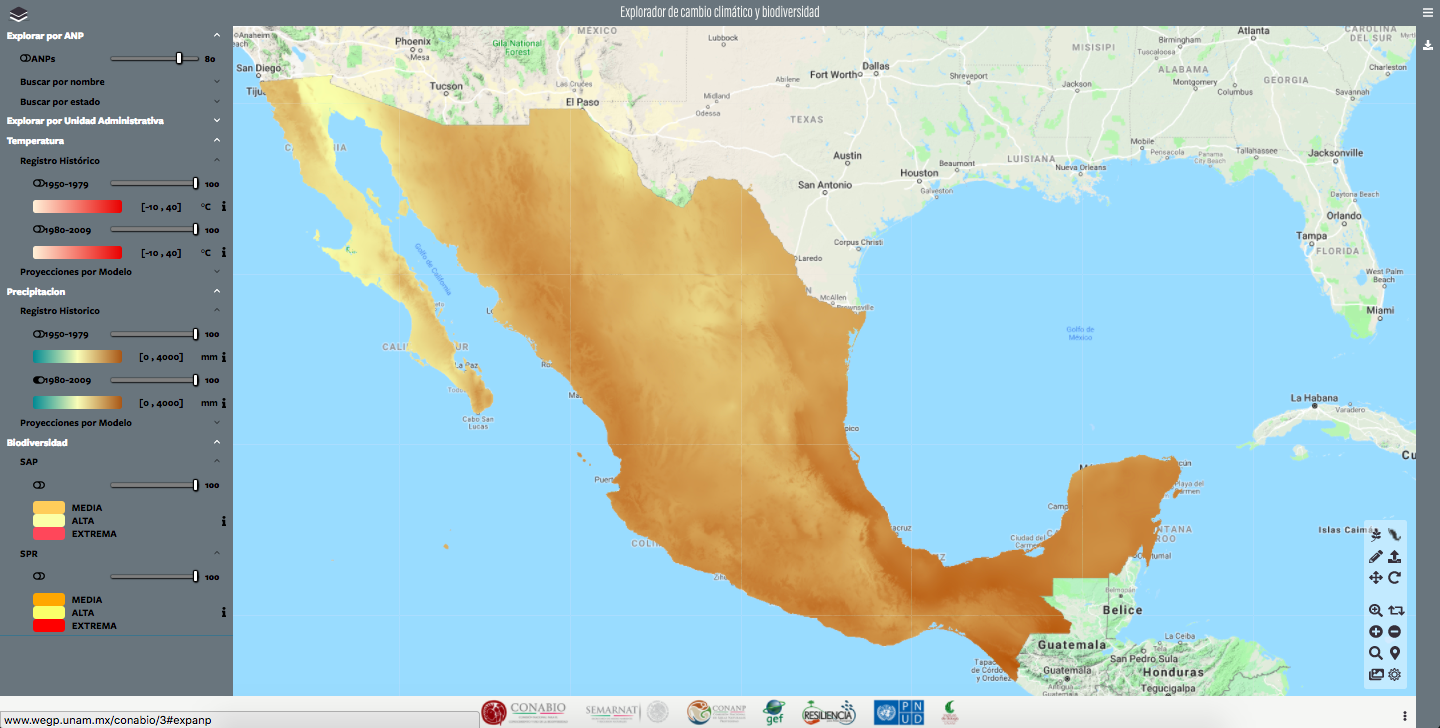
\includegraphics[width=0.9\linewidth]{./logos/entry.png} \\

% 	\textbf{Proyecto financiado por: } \\

	\begin{table}[h!]
	\centering
		%\begin{center}
			\begin{tabular}{ccccc}

				%\multicolumn{3}{c}{
\includegraphics[width=6cm]{./logos/conabio.png}} \\ 
				%
\includegraphics[width=4cm]{./logos/semarnat.png} &
				%
\includegraphics[width=4cm]{./logos/conanp.png} &
				%
\includegraphics[height=2.5cm]{./logos/gef.png} \\

				%
\includegraphics[width=4cm]{./logos/resiliencia.png} &
				%
\includegraphics[width=4cm]{./logos/pnud.png} &
				%
\includegraphics[height=2.5cm]{./logos/unam.png}


				
\includegraphics[width=3cm]{./logos/conabio.png} &
				
\includegraphics[height=2.5cm]{./logos/unam.png} &
				
\includegraphics[width=3cm]{./logos/semarnat.png} &
				
\includegraphics[width=3cm]{./logos/conanp.png} &
				
\includegraphics[width=3cm]{./logos/logoINECC.png} \\

				%\multicolumn{2}{c}{
\includegraphics[height=2.5cm]{./logos/gef.png}} &
				%\multicolumn{2}{c}{
\includegraphics[width=3cm]{./logos/resiliencia.png}} &
				%
\includegraphics[width=3cm]{./logos/pnud.png}

				\multicolumn{2}{c}{
\includegraphics[height=2.5cm]{./logos/gef.png}} &
				\multicolumn{1}{c}{
\includegraphics[width=3cm]{./logos/resiliencia.png}} &
				\multicolumn{2}{c}{
\includegraphics[width=3cm]{./logos/pnud.png}}


			\end{tabular}
		%\begin{center}
	\end{table}
	%\bigskip
	%\bigskip
	\vspace{2.5cm}
	\huge{\textbf{EXPLORADOR DE CAMBIO CLIM\'ATICO Y BIODIVERSIDAD }}\\
	%\bigskip
	\large{COMISI\'ON NACIONAL PARA EL CONOCIMIENTO Y USO DE LA BIODIVERSIDAD \\
	(CONABIO)} \\

	\vspace{2.5cm}

	\textbf{Reporte de la consulta de \'areas inter\'es'} \\
	Reporte generado autom\'aticamente que resume datos de la consulta realizada en
	el \emph{Explorador de cambio clim\'atico y biodiversidad}.
	%\bigskip
	%\bigskip
	%\bigskip
	\vspace{2cm}
	%\small{Conabio, IB-UNAM, Conanp, PNUD, INECC, Reporte de \'areas seleccionadas. Explorador de cambio clim\'atico y biodiversidad. Comisi\'on Nacional para el Conocimiento y Uso de la Biodiversidad, en \ref{http://www.biodiversidad.gob.mx/pais/cambio_climatico.html} Fecha de consulta: }
	%\pagebreak

\end{center}

% \HRule \\[0.25cm]
% { 
% 	\huge \bfseries Summary Report for %\input{../LULCC/TempTables/Country.txt}}
% }
% \HRule \\[0.25cm]
% {
% 	\emph{\large This is an automated report generated by The present document summarizes main results of the model for the red polygon in the map shown here below.\\ } 
% }


% %\includegraphics[width=0.9\linewidth]{../OutBaU/png/Area_of_Interest}

% \textbf{Project funded by:}\\
% %\includegraphics[width=0.2\linewidth]{../LULCC/Wizard_imgs/GACC}
% \end{center}


% \pagebreak 
% %\setlength{\parindent}{0cm}

% \begin{flushleft}

% %A. Ghilardi, R. Bailis, J-F. Mas, R. Drigo, O. Masera. \textbf{Summary Report for \input{../LULCC/TempTables/Country.txt}}- Spatiotemporal modeling of fuelwood environmental impacts. \the\year. CIGA-UNAM and SEI-US. \pageref{lastpage} p.
% \bigskip

\begin{flushleft}
\small{Conabio, IB-UNAM, Conanp, PNUD, INECC, Reporte de \'areas seleccionadas. Explorador de cambio clim\'atico y biodiversidad. Comisi\'on Nacional para el Conocimiento y Uso de la Biodiversidad, en \url{http://www.biodiversidad.gob.mx/pais/cambio_climatico.html} Fecha de consulta: \input{fecha.txt}}
% Comisi\'on Nacional para el Conocimiento y Uso de la Biodiversidad (CONABIO) \\
% Liga Perif\'erico - Insurgentes Sur 4903, \\
% Parques del Pedregal, Del. Tlalpan, \\
% Ciudad de M\'exico. C.P. 14010 \\
% Tel: 5004.5000 \\
% Web: www.gob.mx/conabio
\bigskip
\end{flushleft}

% Centro de Investigaciones en Geografía Ambiental \\
% Universidad Nacional Autónoma de México \\
% Antigua carretera a Pátzcuaro 8701, \\
% Col. Exhacienda de San José de la Huerta, \\
% Morelia, Michoacán, C.P. 58190, Mexico. \\
% Tel: +52 443-322-3854 \\
% Web: www.ciga.unam.mx
% \bigskip

% Stockholm Environment Institute - US Centre \\
% 11 Curtis Ave, \\
% Somerville, MA 02144, United States. \\
% Phone: +1 617-627-3786 \\
% Web: www.sei-us.org
% \bigskip

% Author contact: Adrian Ghilardi, \\
% Centro de Investigaciones en Geografía Ambiental, \\
% Universidad Nacional Autónoma de México. \\
% aghilardi@ciga.unam.mx
% \bigskip \bigskip \bigskip \bigskip \bigskip \bigskip \bigskip \bigskip

% %Cover Photo: Cow dung drying in Haryana, Northern India, for
% %use as a domestic energy source amongst rural households.
% %© Adrian Ghilardi
% %\\[3.0cm]

% This publication may be reproduced in whole or in part and in any
% form for educational or non-profit purposes, without special permission
% from the copyright holder(s) provided acknowledgement
% of the source is made. No use of this publication may be made for
% resale or other commercial purpose, without the written permission
% of the copyright holder(s).
% \bigskip


% %\includegraphics[width=0.1\linewidth]{../LULCC/Wizard_imgs/SEI}

% \end{flushleft}
\end{titlepage}
	
	\section*{Acerca de este reporte}
	%% El Explorador de cambio clim\'atico y biodiversidad (ECCBio) \footnote{Esta herramienta se basa en el trabajo financiado por el proyecto \emph{Fortalecimiento de la efectividad del manejo y la resiliencia de las \'Areas Protegidas para proteger la biodiversidad amenazada por el Cambio Clim\'atico}} es una herramienta de consulta en l\'inea sobre las tendencias del cambio clim\'atico global en M\'exico y sus posibles efectos en varios elementos de la diversidad biol\'ogica. En el ECCBio es posible visualizar diversas capas de informaci\'on, como las \'areas expuestas a mayores cambios en el clima que, por ende, ser\'an m\'as vulnerables; las \'areas que probablemente permanecer\'an estables y que podr\'ian ser utilizadas por distintas especies como refugios para persistir en el futuro; as\'i como \'areas que presentan p\'erdida de las condiciones ambientales actuales en las que subsiste.

	El Explorador de cambio clim\'atico y biodiversidad (ECCBio)1 es una herramienta de consulta en l\'inea sobre las tendencias del cambio clim\'atico global en M\'exico y sus posibles efectos en varios elementos de la diversidad biol\'ogica. El ECCBio permite explorar las tendencias de cambio en las condiciones clim\'aticas de 1950 a 2099, bajo distintos escenarios de cambio clim\'atico; el estado de conectividad estructural de la vegetaci\'on natural en las \'areas naturales protegidas terrestres del pa\'is; y el grado de conectividad entre las \'areas naturales protegidas. 

	En el ECCBio es posible visualizar diversas capas de informaci\'on, como las \'areasexpuestas a mayores cambios en el clima y que, por ende, ser\'an m\'as vulnerables; las \'areas que probablemente permanecer\'an estables y que podr\'ian ser utilizadas por distintas especies como refugios para persistir en el futuro; as\'i como \'areas que presentan p\'erdida de las condiciones ambientales actuales en las que subsiste un conjunto de especies, y las \'areas que potencialmente podr\'ian llegar a colonizar ante los cambios proyectados en el clima; y los corredores clim\'aticos, una de las estrategias de conservaci\'on frecuentemente recomendadas para mantener la resiliencia de los ecosistemas y contribuir a la conservaci\'on de la biodiversidad ante las tendencias del cambio global.

	En este reporte se presentan los datos y gr\'aficas asociadas a las consultas de las tendencias de cambio de las condiciones clim\'aticas (temperatura y precipitaci\'on) de 1950 a 2099, bajo distintos escenarios de cambio clim\'atico, en las \'areas naturales protegidas terrestres, municipios, estados o en cualquier \'area del pa\'is predefinida por el usuario. Asimismo, se presentan an\'alisis e indicadores sobre el estado de la conectividad del paisaje en las \'areas naturales protegidas terrestres y la conectividad entre dichas \'areas, lo que brinda herramientas que contribuyen a evaluar la Meta 11 de Aichi del Convenio sobre la Diversidad Biol\'ogica (CDB).

	El ECCBio permite consultar los diferentes escenarios de cambio clim\'atico que corresponden a cuatro modelos de circulaci\'on global: MPI-ESM-LR (Alemania), GFDL-CM3 (Estados Unidos), HADGEM2-ES (Reino Unido) y CNRMCM5 (Francia) y dos trayectorias de concentraciones representativas (RCP, por sus siglas en ingl\'es) que proyectan las condiciones clim\'aticas en el futuro para los per\'iodos de 2015 a 2039, 2045 a 2069 y de 2075 a 2099. Las proyecciones, que describen cuatro trayectorias distintas en el siglo XXI, se basan en los factores que determinan las emisiones de gases de efecto invernadero, tales como el tama\~no de la poblaci\'on, la actividad econ\'omica, el estilo de vida, la p\'erdida y degradaci\'on de la vegetaci\'on natural y la pol\'itica clim\'atica. En el ECCBio se utilizan dos RCP; la trayectoria RCP 4.5 y 8.5 que corresponden respectivamente a escenarios con un nivel moderado y muy alto de emisiones de gases de efecto invernadero.


	\newpage
	\tableofcontents

	% \pretitle{%
	% 	\begin{center}
	% 	
\includegraphics[width=7.5cm]{./conabio.png}\\[\bigskipamount]
	% }

	% \title{Explorador de cambio clim\'atico y Biodiversidad}
	% \author{Comisi\'on Nacional para el Conocimiento y Uso de la Biodiversidad (CONABIO)}



	% \maketitle
	% \tableofcontents
	% %\listoffigures

	% \begin{figure}[!ht]
	% 	\centering
	% 	
\includegraphics[width=9.5cm,height=4cm]{./conabio.png}
	% \end{figure}


	% \section{Acerca de este Reporte}

	% La \emph{CONABIO} tiene la misi\'onN de promover, coordinar, apoyar y realizar actividades dirigidas al conocimiento de la diversidad biol\'ogica, así como a su conservaci\'on y uso sustentable para beneficio de la sociedad. Fue concebida como una organizaci\'on de investigaci\'on aplicada, promotora de investigaci\'on básica, que compila y genera informaci\'on sobre biodiversidad, desarrolla capacidades humanas en el área de informática de la biodiversidad y es fuente pública de informaci\'on y conocimiento accesible para toda la sociedad.

	\section*{Resultados}
	\begin{python}
		# -*- coding: UTF8 -*- 
		import os
		import codecs
		
		directory = "./"
		extension = ".csv"
		files = [file for file in os.listdir(directory) if file.lower().endswith(extension)]

		t = open(directory+"tipo.txt","r")
		tipo = t.read()
		t.close()

		for file in files:
		   csv = file[0]+".csv"
		   tit = directory+"titulo"+file[0]+".txt"
		   f = open(tit, "r")
		   nombre = f.read()
		   f.close()
		   tit = directory+"tituloNombre"+file[0]+".txt"
		   f = open(tit, "r")
		   nombreCompleto = f.read()
		   f.close()
		   tit = directory+"tituloCategoria"+file[0]+".txt"
		   f = open(tit, "r")
		   nombreCategoria = f.read()
		   f.close()
		   nombreCompleto = nombreCategoria+" "+nombreCompleto

		   print r"\pagebreak"
		   # if(file[0] == '1'):
		      # print r"\section{Resultados}"
		   # print r"\section{%s}" % nombre
		   print r"\section{%s}" % nombreCompleto
		   # print r"%s}" % nombreCompleto

		   nombreCaption = directory+"caption"+file[0]+".txt"
		   caption = open(nombreCaption, "r")
		   variable = caption.readline()[:-1]
		   periodo = caption.readline()[:-1]
		   caption.close()

		   
		   if(tipo[0] == '0'):
		      inf = directory+"info"+file[0]+".txt"
		      i = open(inf, 'r')
		      cadMedia = 'infoMedia'+file[0]+'.txt'
		      cadMax = 'infoMax'+file[0]+'.txt'
		      cadMin = 'infoMin'+file[0]+'.txt'
		      cadPrec = 'infoPrec'+file[0]+'.txt'

		      print r"\subsection{Clima al presente}"
		      print r"\begin{table}[H]"
		      print r"\begin{tabular}{crc}"
		      print r"\multirow{3}{*}{
\includegraphics[height=1.15cm]{./logos/icon-thermometer.png}} & media &  \input{%s} $^{\circ}$C\\" %cadMedia
		      print r"                & maxima & \input{%s} $^{\circ}$C \\" %cadMax
		      print r"                & minima & \input{%s} $^{\circ}$C \\" %cadMin
		      print r"
\includegraphics[height=0.8cm]{./logos/icon-drop.png}&   \input{%s} mm     & " %cadPrec
		      print r"\end{tabular}"
		      print r"\end{table}"

		      print r"\subsection{Clima a futuro}"
		      print r"\begin{table}[H]"
		      print r"\begin{tabular}{c}"
		      print r"\multirow{3}{*}{
\includegraphics[height=1.15cm]{./logos/climafuturo.png}}"
		      print r"\end{tabular}"
		      print r"\end{table}"

		      print r"Se refiere al grado en el que las variaciones clim\'aticas afectan a los ecosistemas; una mayor exposici\'on podr\'ia incrementar la vulnerabilidad de los mismos. Para el \'area de inter\'es (\'area protegida, estado, municipio o pol\'igono) se reporta la proporci\'on de superficie en la que coinciden los cuatro modelos de circulaci\'on global (MCG): MPI-ESM-LR (Alemania), GFDL-CM3 (Estados Unidos), HADGEM2-ES (Reino Unido) y CNRMCM5 (Francia). Se presentan dos gr\'aficas que son complementarias; La gr\'afica circular corresponde a la proporci\'on de la superficie que se estima permanecer\'a con condiciones clim\'aticas estables, lo que fue identificado a partir de la delimitaci\'on de las zonas de vida de Holdridge, utilizando variables bioclim\'aticas (biotemperatura, precipitaci\'on y el potencial de evapotranspiraci\'on) para el segundo periodo hist\'orico (1980 a 2009; \cite{Cuervo191}) y los tres horizontes futuros bajo los cuatro MCG con escenarios de emisiones RCP 4.5 y 8.5 (moderado y muy alto, respectivamente). La gr\'afica de barras muestra la proporci\'on de la superficie del \'area de inter\'es que potencialmente presentar\'a un incremento significativo y constante de la temperatura media, considerando del periodo m\'as antiguo (1950-1979; \cite{Cuervo19}) al periodo futuro m\'as lejano (2075-2099) con base en los escenarios de cambio clim\'atico \cite{Fernandez15}. Las \'areas que no cambian respecto a sus zonas de vida son consideradas estables. Note que cuando elige un periodo futuro m\'as alejado o un escenario de emisiones m\'as alto, el porcentaje de \'area disminuye."

		      print r"\begin{figure}[H]"
		      print r"\centering"
		      print r"\includegraphics[trim= 0 0 0 80, clip, width=11cm,height=10cm]{%s}" % (directory+file[0]+'E')
		      print r"\caption{Proporci\'on de la superficie del \'area de inter\'es que mantiene las condiciones clim\'aticas (zonas de vida estables) para el periodo.}"
		      print r"\end{figure}"
		      
		      print r"\begin{figure}[H]"
		      print r"\centering"
		      print r"\includegraphics[trim= 0 0 0 80, clip, width=11cm,height=10cm]{%s}" % (directory+file[0]+'Mann')
		      print r"\caption{Proporci\'on de la superficie terrestre del \'area de inter\'es con incremento constante de la temperatura media (rojo).}"
		      print r"\end{figure}"

		      nombreTabla = directory+"infoTabla"+file[0]+".txt"
		      infoTabla = open(nombreTabla, "r")
		      rl = infoTabla.readline()[:-1]
		      
		      print r"\begin{table}[H]"
		      print r"\caption{Cambios proyectados respecto al promedio hist\'orico: intervalo de variaci\'on entre los cuatro modelos de circulaci\'on global}"
		      print r"\begin{tabular}{cccc}"
		      print r"&Periodo& RCP 4.5 & RCP 8.5 \\"
		      print r"\multirow{6}{*}{\textcolor{brown}{Temperatura m\'inima ($^{\circ}$C)}} & \multirow{2}{*}{2015-2039} & \multirow{2}{*}{"
		      print r"(%s" %rl
		      rl = infoTabla.readline()[:-1]
		      print r" , %s)" %rl
		      rl = infoTabla.readline()[:-1]
		      print r"}  & \multirow{2}{*}{(%s" %rl
		      rl = infoTabla.readline()[:-1]
		      print r" , %s)}   \\" %rl
		      print r" & & & \\"
		      rl = infoTabla.readline()[:-1]
		      print r"                                    & \multirow{2}{*}{2045-2069} & \multirow{2}{*}{(%s" %rl
		      rl = infoTabla.readline()[:-1]
		      print r" , %s)}  & \multirow{2}{*}{" %rl
		      rl = infoTabla.readline()[:-1]
		      print r"(%s , " %rl
		      rl = infoTabla.readline()[:-1]
		      print r"%s)}   \\" %rl
		      print r" & & & \\"
		      rl = infoTabla.readline()[:-1]
		      print r"                                    & \multirow{2}{*}{2075-2099} & \multirow{2}{*}{(%s" %rl
		      rl = infoTabla.readline()[:-1]
		      print r" , %s)}" %rl
		      rl = infoTabla.readline()[:-1]
		      print r" & \multirow{2}{*}{(%s" %rl
		      rl = infoTabla.readline()[:-1]
		      print r" , %s)} \\" %rl
		      print r" & & & \\"
		      rl = infoTabla.readline()[:-1]
		      print r"\multirow{6}{*}{\textcolor{orange}{Temperatura media ($^{\circ}$C)}} & \multirow{2}{*}{2015-2039} & \multirow{2}{*}{(%s" %rl
		      rl = infoTabla.readline()[:-1]
		      print r" , %s)" %rl
		      rl = infoTabla.readline()[:-1]
		      print r"}  & \multirow{2}{*}{(%s" %rl
		      rl = infoTabla.readline()[:-1]
		      print r" , %s)}   \\" %rl
		      print r" & & & \\"
		      rl = infoTabla.readline()[:-1]
		      print r"                                    & \multirow{2}{*}{2045-2069} & \multirow{2}{*}{(%s" %rl
		      rl = infoTabla.readline()[:-1]
		      print r" , %s)}  & \multirow{2}{*}{" %rl
		      rl = infoTabla.readline()[:-1]
		      print r"(%s , " %rl
		      rl = infoTabla.readline()[:-1]
		      print r"%s)}   \\" %rl
		      print r" & & & \\"
		      rl = infoTabla.readline()[:-1]
		      print r"                                    & \multirow{2}{*}{2075-2099} & \multirow{2}{*}{(%s" %rl
		      rl = infoTabla.readline()[:-1]
		      print r" , %s)}" %rl
		      rl = infoTabla.readline()[:-1]
		      print r" & \multirow{2}{*}{(%s" %rl
		      rl = infoTabla.readline()[:-1]
		      print r" , %s)} \\" %rl
		      print r" & & & \\"
		      rl = infoTabla.readline()[:-1]
		      print r"\multirow{6}{*}{\textcolor{red2}{Temperatura m\'axima ($^{\circ}$C)}} & \multirow{2}{*}{2015-2039} & \multirow{2}{*}{(%s" %rl
		      rl = infoTabla.readline()[:-1]
		      print r" , %s)" %rl
		      rl = infoTabla.readline()[:-1]
		      print r"}  & \multirow{2}{*}{(%s" %rl
		      rl = infoTabla.readline()[:-1]
		      print r" , %s)}   \\" %rl
		      rl = infoTabla.readline()[:-1]
		      print r" & & & \\"
		      # rl = infoTabla.readline()[:-1]
		      print r"                                    & \multirow{2}{*}{2045-2069} & \multirow{2}{*}{(%s" %rl
		      rl = infoTabla.readline()[:-1]
		      print r" , %s)}  & \multirow{2}{*}{" %rl
		      rl = infoTabla.readline()[:-1]
		      print r"(%s , " %rl
		      rl = infoTabla.readline()[:-1]
		      print r"%s)}   \\" %rl
		      print r" & & & \\"
		      rl = infoTabla.readline()[:-1]
		      print r"                                    & \multirow{2}{*}{2075-2099} & \multirow{2}{*}{(%s" %rl
		      rl = infoTabla.readline()[:-1]
		      print r" , %s)}" %rl
		      rl = infoTabla.readline()[:-1]
		      print r" & \multirow{2}{*}{(%s" %rl
		      rl = infoTabla.readline()[:-1]
		      print r" , %s)} \\" %rl
		      print r" & & & \\"
		      rl = infoTabla.readline()[:-1]
		      print r"\multirow{6}{*}{\textcolor{blue}{Precipitaci\'on total (mm) }\textcolor{grey}{(o/o)}} & \multirow{2}{*}{2015-2039} & (%s" %rl
		      rl = infoTabla.readline()[:-1]
		      print r" , %s)" %rl
		      rl = infoTabla.readline()[:-1]
		      print r"   & (%s" %rl
		      rl = infoTabla.readline()[:-1]
		      print r" , %s)   \\" %rl
		      rl = infoTabla.readline()[:-1]
		      print r"                                    &                            & \textcolor{grey}{(%s}" %rl
		      rl = infoTabla.readline()[:-1]
		      print r" , \textcolor{grey}{%s)}" %rl
		      rl = infoTabla.readline()[:-1]
		      print r"   & \textcolor{grey}{(%s}" %rl
		      rl = infoTabla.readline()[:-1]
		      print r" , \textcolor{grey}{%s)}   \\" %rl
		      rl = infoTabla.readline()[:-1]
		      print r"                                    & \multirow{2}{*}{2045-2069} & (%s" %rl
		      rl = infoTabla.readline()[:-1]
		      print r" , %s)  & " %rl
		      rl = infoTabla.readline()[:-1]
		      print r"(%s , " %rl
		      rl = infoTabla.readline()[:-1]
		      print r"%s) \\" %rl
		      rl = infoTabla.readline()[:-1]
		      print r"                                    &                            & \textcolor{grey}{(%s}" %rl
		      print r" , "
		      rl = infoTabla.readline()[:-1]
		      print r"\textcolor{grey}{%s)} & " %rl
		      rl = infoTabla.readline()[:-1]
		      print r"\textcolor{grey}{(%s} , " %rl
		      rl = infoTabla.readline()[:-1]
		      print r"\textcolor{grey}{%s)} \\" %rl
		      rl = infoTabla.readline()[:-1]
		      print r"                                    & \multirow{2}{*}{2075-2099} & (%s" %rl
		      rl = infoTabla.readline()[:-1]
		      print r" , %s) & " %rl
		      rl = infoTabla.readline()[:-1]
		      print r"(%s , " %rl
		      rl = infoTabla.readline()[:-1]
		      print r"%s) \\" %rl
		      rl = infoTabla.readline()[:-1]
		      print r"                                    &                            & \textcolor{grey}{(%s}" %rl
		      rl = infoTabla.readline()[:-1]
		      print r" , \textcolor{grey}{%s)} & " %rl
		      rl = infoTabla.readline()[:-1]
		      print r"\textcolor{grey}{(%s} , " %rl
		      rl = infoTabla.readline()[:-1]
		      print r"\textcolor{grey}{%s)}" %rl
		      print r"\end{tabular}"
		      print r"\end{table}"
		      infoTabla.close()


		      # print r"\bf{Cambio proyectado (RCP 8.5)\\}"
		      
		      var = i.readline()
		      if(float(var[:4]) >= 0):
		         cad = "exceder\\'a"
		      else:
		         cad = "disminuir\\'a"
		      # print r"La \textcolor{red}{temperatura m\'axima} en el ANP %s el promedio historico por:\\" % cad
		      
		      # print r"\begin{itemize}"
		      # print r"\setlength\itemsep{1em}"
		      # print r"\item[*] %s  $^\circ$C para el periodo 2015-2039\\" % var
		      var = i.readline()
		      # print r"\item[*] %s  $^\circ$C para el periodo 2075-2099\\" % var
		      # print r"\end{itemize}"

		      var = i.readline()
		      if(float(var[:4]) >= 0):
		         cad = "exceder\\'a"
		      else:
		         cad = "disminuir\\'x"
		      # print r"La \textcolor{yellow}{temperatura m\'inima} en el ANP %s el promedio historico por:\\" % cad
		      # print r"\begin{itemize}"
		      # print r"\setlength\itemsep{0em}"
		      # print r"\item[*] %s  $^\circ$C para el periodo 2015-2039\\" % var
		      var = i.readline()
		      # print r"\item[*] %s  $^\circ$C para el periodo 2075-2099\\" % var
		      # print r"\end{itemize}"

		      var = i.readline()
		      if(float(var[:4]) >= 0):
		         cad = "exceder\\'a"
		      else:
		         cad = "disminuir\\'a"
		      # print r"La \textcolor{blue}{precipitaci\'on promedio} en el ANP %s el promedio historico por:\\" % cad
		      # print r"\begin{itemize}"
		      # print r"\item[*] %s  $^\circ$C para el periodo 2015-2039\\" % var
		      var = i.readline()
		      # print r"\item[*] %s  $^\circ$C para el periodo 2075-2099\\" % var
		      # print r"\end{itemize}"
		      i.close()
		   else:
		      print r""

		   nombreYears = directory+"years"+file[0]+".txt"
		   years = open(nombreYears, "r")
		   rl = years.readline()[:-1]

		   if(variable == 'Temperatura mínima'):
		      plural = 'Temperaturas mínimas'
		   elif(variable == 'Temperatura máxima'):
		      plural = 'Temperaturas máximas'
		   elif(variable == 'Precipitaci\'on total'):
		      plural = 'Precipitaciones totales'
		   elif(variable == 'Temperatura media'):
		      plural = 'Temperaturas medias'
		   else:
		      plural = variable

		   print r"\begin{table}[H]"
		   print r"\caption{%s " %plural 
		   print r"anuales para los periodos hist\'oricos y los cuatro modelos de circulaci\'on global}"
		   print r"\begin{tabular}{lcccccc}"
		   print r"\cline{2-7}"
		   print r"&\multicolumn{6}{c}{\textbf{Modelos}} \\ \hline"
		   print r"& Historico & CNRMCM5 & MPI\_ESM\_LR &  HADGEM2\_ES & GFDL\_CM3 & Promedio* \\ \hline"
		   
		   print r"1950-1979 & %s & - & - & - & - & -\\" %rl
		   rl = years.readline()[:-1]
		   print r"1980-2009 & %s & -  & -  & -  & -  & -\\" %rl
		   
		   rl = years.readline()[:-1]
		   print r"2015-2039 (RCP 4.5) & -  & %s " %rl
		   rl = years.readline()[:-1]
		   print r"& %s " %rl
		   rl = years.readline()[:-1]
		   print r"& %s " %rl
		   rl = years.readline()[:-1]
		   print r"& %s " %rl
		   rl = years.readline()[:-1]
		   print r"& %s \\" %rl

		   rl = years.readline()[:-1]
		   print r"2015-2039 (RCP 8.5) & -  & %s " %rl
		   rl = years.readline()[:-1]
		   print r"& %s " %rl
		   rl = years.readline()[:-1]
		   print r"& %s " %rl
		   rl = years.readline()[:-1]
		   print r"& %s " %rl
		   rl = years.readline()[:-1]
		   print r"& %s \\" %rl

		   rl = years.readline()[:-1]
		   print r"2045-2069 (RCP 4.5) & -  & %s " %rl
		   rl = years.readline()[:-1]
		   print r"& %s " %rl
		   rl = years.readline()[:-1]
		   print r"& %s " %rl
		   rl = years.readline()[:-1]
		   print r"& %s " %rl
		   rl = years.readline()[:-1]
		   print r"& %s \\" %rl

		   rl = years.readline()[:-1]
		   print r"2045-2069 (RCP 8.5) & -  & %s " %rl
		   rl = years.readline()[:-1]
		   print r"& %s " %rl
		   rl = years.readline()[:-1]
		   print r"& %s " %rl
		   rl = years.readline()[:-1]
		   print r"& %s " %rl
		   rl = years.readline()[:-1]
		   print r"& %s \\" %rl

		   rl = years.readline()[:-1]
		   print r"2075-2099 (RCP 4.5) & -  & %s " %rl
		   rl = years.readline()[:-1]
		   print r"& %s " %rl
		   rl = years.readline()[:-1]
		   print r"& %s " %rl
		   rl = years.readline()[:-1]
		   print r"& %s " %rl
		   rl = years.readline()[:-1]
		   print r"& %s \\" %rl

		   rl = years.readline()[:-1]
		   print r"2075-2099 (RCP 8.5) & -  & %s " %rl
		   rl = years.readline()[:-1]
		   print r"& %s " %rl
		   rl = years.readline()[:-1]
		   print r"& %s " %rl
		   rl = years.readline()[:-1]
		   print r"& %s " %rl
		   rl = years.readline()[:-1]
		   print r"& %s \\ \hline" %rl
		   
		   print r"& \multicolumn{1}{l}{} & \multicolumn{1}{l}{} & \multicolumn{1}{l}{} & \multicolumn{1}{l}{} & \multicolumn{1}{l}{} & \multicolumn{1}{l}{}"
		   print r"\end{tabular}"
		   print r"\end{table}"
			  

		   # nombreCaption = directory+"caption"+file[0]+".txt"
		   # caption = open(nombreCaption, "r")
		   # variable = caption.readline()[:-1]
		   # periodo = caption.readline()[:-1]
		   # caption.close()

		   print r"\begin{figure}[H]"
		   print r"\centering"
		   print r"\includegraphics[trim= 0 0 0 80, clip, width=11cm,height=10cm]{%s}" % (directory+file[0]+'N')
		   print r"\caption{Valores promedio de en el \'area de inter\'es para la  %s" %variable
		   print r" en el periodo %s}" %periodo
		   print r"\end{figure}"

		   nombreCaption2 = directory+"caption2"+file[0]+".txt"
		   caption2 = open(nombreCaption2, "r")
		   variable2 = caption2.readline()[:-1]
		   periodo2 = caption2.readline()[:-1]
		   modelo2 = caption2.readline()[:-1]
		   forz2 = caption2.readline()[:-1]
		   caption2.close()

		   # print "modelo: ", modelo2
		   # print "forza: ", forz2

		   print r"\begin{figure}[H]"
		   print r"\centering"
		   print r"\includegraphics[trim= 0 0 0 80, clip, width=11cm,height=10cm]{%s}" % (directory+file[0])
		   print r"\caption{Dispersi\'on de la %s" % variable2
		   print r" para el periodo %s" %periodo2
		   print r" con el modelo %s" %modelo2
		   print r" y RCP %s}" %forz2
		   print r"\end{figure}"

		   nombreStatics = directory+"statics"+file[0]+".txt"
		   statics = open(nombreStatics, "r")
		   
		   print r"\begin{center}"
		   print r"\begin{table}[H]"
		   print r"\caption{Mediana, valor m\'inimo y valor m\'aximo para la %s " %variable2
		   print r"en el periodo %s " %periodo2
		   print r"para el modelo %s " %modelo2
		   print r"con forzamiento %s}" %forz2 
		   print r"\begin{tabular}{cccc}"
		   print r"\hline"
		   print r"          & Mediana & Valor m\'inimo & Valor m\'aximo \\ \hline"
		   rl = statics.readline()[:-1]
		   print r"1950-1979 & %s     &" %rl
		   rl = statics.readline()[:-1]
		   # print r" %s & " %rl
		   rl = statics.readline()[:-1]
		   # print r" %s & " %rl
		   rl = statics.readline()[:-1]
		   print r" %s & " %rl
		   rl = statics.readline()[:-1]
		   print r" %s          \\" %rl
		   rl = statics.readline()[:-1]
		   print r"1980-2009 & %s     &" %rl
		   rl = statics.readline()[:-1]
		   # print r" %s & " %rl
		   rl = statics.readline()[:-1]
		   # print r" %s & " %rl
		   rl = statics.readline()[:-1]
		   print r" %s & " %rl
		   rl = statics.readline()[:-1]
		   print r" %s          \\" %rl
		   rl = statics.readline()[:-1]
		   print r"2015-2039 & %s     &" %rl
		   rl = statics.readline()[:-1]
		   # print r" %s & " %rl
		   rl = statics.readline()[:-1]
		   # print r" %s & " %rl
		   rl = statics.readline()[:-1]
		   print r" %s & " %rl
		   rl = statics.readline()[:-1]
		   print r" %s          \\" %rl
		   rl = statics.readline()[:-1]
		   print r"2045-2069 & %s     &" %rl
		   rl = statics.readline()[:-1]
		   # print r" %s & " %rl
		   rl = statics.readline()[:-1]
		   # print r" %s & " %rl
		   rl = statics.readline()[:-1]
		   print r" %s & " %rl
		   rl = statics.readline()[:-1]
		   print r" %s          \\" %rl
		   rl = statics.readline()[:-1]
		   print r"2075-2099 & %s     &" %rl
		   rl = statics.readline()[:-1]
		   # print r" %s & " %rl
		   rl = statics.readline()[:-1]
		   # print r" %s & " %rl
		   rl = statics.readline()[:-1]
		   print r" %s & " %rl
		   rl = statics.readline()[:-1]
		   print r" %s          \\ \hline" %rl
		   print r"\end{tabular}"
		   print r"\end{table}"
		   print r"\end{center}"
		   statics.close()

		   print r"\subsection{Conectividad}"
		   print r"\begin{table}[H]"
		   print r"\begin{tabular}{c}"
		   print r"\multirow{3}{*}{
\includegraphics[height=1.15cm]{./logos/conectividad.png}}"
		   print r"\end{tabular}"
		   print r"\end{table}"

		   print r"\subsubsection{\'Indice de Fragmentaci\'on}"
		   print r"El \'indice de fragmentaci\'on mide el grado de fragmentaci\'on de la vegetaci\'on primaria y secundaria arb\'orea y considera el impacto generado por el cambio de uso del suelo. La fragmentaci\'on se expresa en porcentaje y su valor ser\'a mayor si existen m\'as barreras como carreteras, \'areas urbanas o tierras agr\'icolas, que puedan dificultar el movimiento de organismos entre fragmentos de vegetaci\'on (\cite{Moser07})."

		   print r"\begin{figure}[H]"
		   print r"\centering"
		   print r"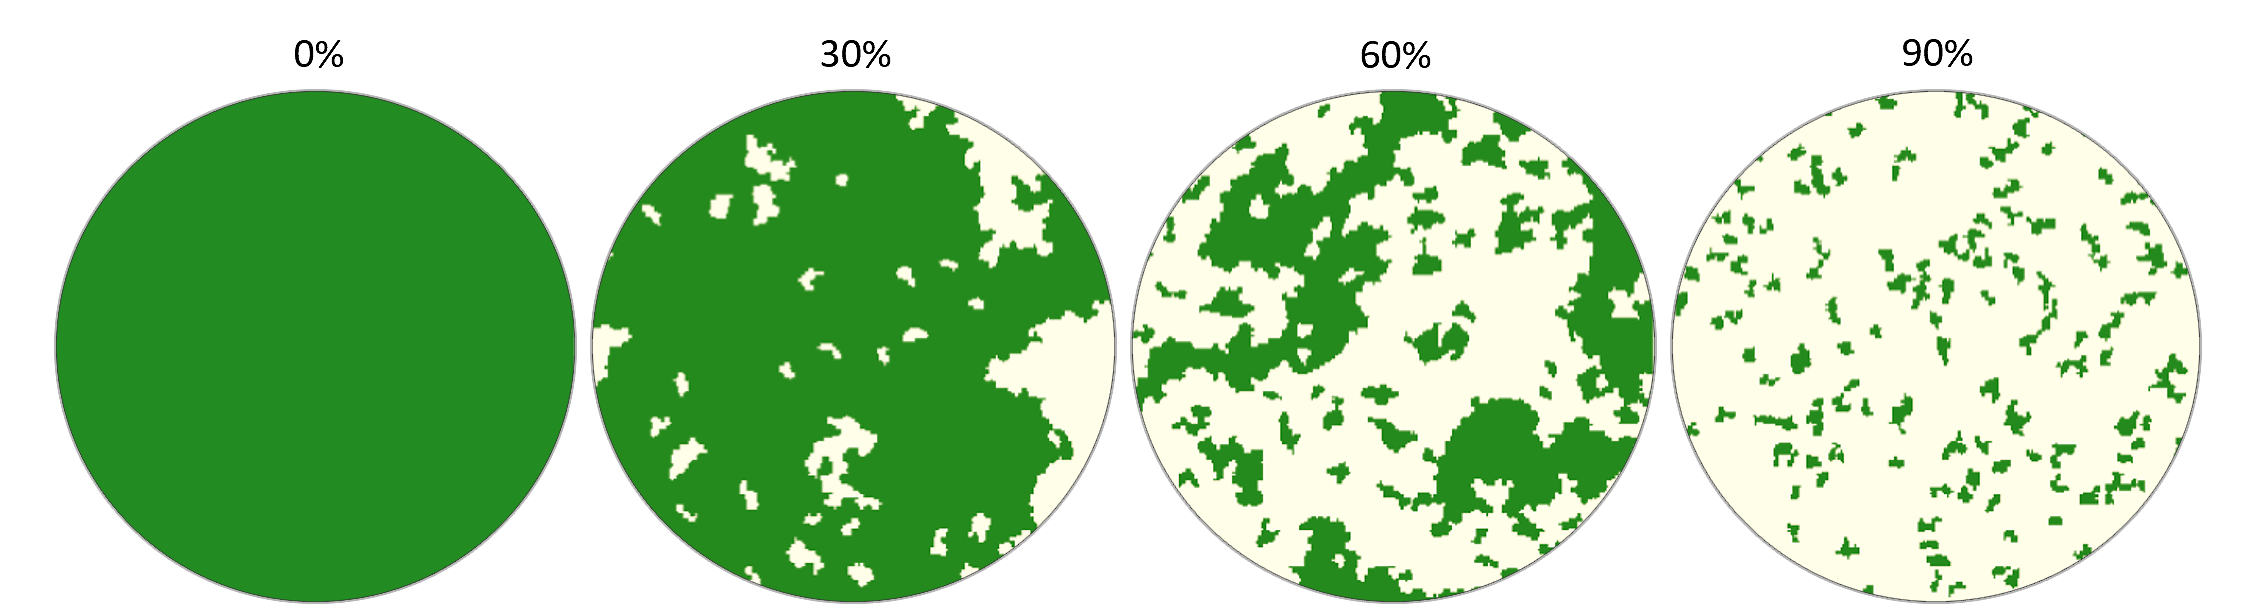
\includegraphics[width=15cm,height=4cm]{./logos/fragmentacionClip.png}"
		   print r"\caption{\'Indice de fragmentaci\'on (\%)}"
		   print r"\end{figure}"

		   print r"El \'indice se calcul\'o para los pol\'igonos de cada una de las \'areas protegidas y para sus zonas de influencia de hasta 10 km (dependiendo de su l\'imite con las costas). La figura inicial sirve para ejemplificar como se ve un paisaje con un valor bajo o alto del \'indice de fragmentaci\'on. As\'i, por ejemplo, si algún \'area protegida tiene un valor del \'indice igual a 0\%, su vegetaci\'on no estar\'ia fragmentada (i.e. se trata de un solo pol\'igono), mientras que un \'area protegida con un valor superior a 90\% indica un gran n\'umero de fragmentos de vegetaci\'on, pequeños y distantes entre s\'i, producto principalmente del cambio de uso del suelo."

		   print r"\begin{figure}[H]"
		   print r"\centering"
		   print r"\includegraphics[trim= 0 0 0 80, clip, width=11cm,height=10cm]{%s}" % (directory+file[0]+'F')
		   print r"\caption{Porcentaje de framentaci\'on de la vegetaci\'on en el \'area protegida}"
		   print r"\end{figure}"

		   print r"\subsubsection{An\'alisis de tendencia temporal de conectividad de la vegetaci\'on}"
		   print r"El an\'alisis de tendencias temporales brinda una estimaci\'on sobre los cambios en la conectividad de los fragmentos de vegetaci\'on por cambio clim\'atico. Se us\'o el \'indice conexo equivalente que incorpora la distancia entre cada par de fragmentos de vegetaci\'on primaria y un atributo que describe su calidad (\cite{Saura11, Saura17}). El \'indice se calcul\'o para los fragmentos de vegetaci\'on primaria de la carta de uso del suelo y vegetaci\'on serie VI (\cite{Inegi2013, Inegi2016}) presentes en las \'areas protegidas y sus zonas de influencia de hasta 10 km (dependiendo de su cercanía a la costa). El atributo de calidad de cada fragmento corresponde a su \'area multiplicada por su grado de estabilidad clim\'atica en tres periodos futuros (2015-2039, 2045-2069 y 2075-2099) para dos escenarios de trayectorias de concentraciones representativas (RCP 4.5 y 8.5). Las distancias entre fragmentos de vegetaci\'on corresponden a las rutas con menor impacto humano; se estimaron usando un \'indice de impacto humano que incorpora tres de los factores de presi\'on antropog\'enicos m\'as importantes: cambio de uso del suelo, desarrollo de infraestructura y fragmentaci\'on de h\'abitats (v\'ease la informaci\'on en el m\'odulo de conectividad del panel izquierdo). La conectividad se expresa en porcentaje y su valor ser\'a mayor en el \'area protegida y su zona de influencia si tiene m\'as fragmentos en donde la mayor parte de su \'area es estable clim\'aticamente y si la distancia entre sus fragmentos es menor a la establecida como la distancia m\'axima de dispersi\'on. El an\'alisis de tendencias de la conectividad en el \'area protegida y su zona de influencia se puede visualizar bajo cuatro distancias que se relacionan con la capacidad de dispersi\'on diferenciada de varios grupos taxon\'omicos como anfibios, reptiles, aves y grandes mam\'iferos (2, 10, 30 y 100 km)."

		   print r"\begin{figure}[H]"
		   print r"\centering"
		   print r"\includegraphics[trim= 0 0 0 80, clip, width=11cm,height=10cm]{%s}" % (directory+file[0]+'T')
		   print r"\caption{Tendencia temporal de conectividad de la vegetaci\'on en el \'area protegida ante el cambio clim\'atico}"
		   print r"\end{figure}"

		   print r"\subsubsection{Conectividad y cobertura de las \'areas protegidas en las ecorregiones terrestres}"
		   print r"El \'indice ProtConn fue dise\~nado para evaluar metas de conservaci\'on tales como la meta 11 de Aichi y cuantifica la conectividad de la red de \'areas protegidas. El \'indice incorpora la superficie y distancia entre las \'areas protegidas. Las distancias entre las \'areas protegidas corresponden a las rutas con menor impacto humano. Las distancias se estimaron usando un \'indice de impacto humano que incorpora tres de los factores de presi\'on antropog\'enicos m\'as importantes: cambio de uso del suelo, desarrollo de infraestructura y fragmentaci\'on de h\'abitats (v\'ease la informaci\'on en el m\'odulo de conectividad del panel izquierdo). El \'indice ProtConn se compone de tres valores que representan una proporci\'on respecto al \'area total de la ecorregi\'on: 1) porcentaje de la ecorregi\'on que no est\'a protegida, ii) porcentaje de la ecorregi\'on que est\'a protegida y iii) porcentaje de la ecorregi\'on que est\'a protegida y conectada. El \'indice ProtConn se calcul\'o para la red de \'areas protegidas de jurisdicci\'on federal (\cite{Semarnat17}) y se puede visualizar para tres de los niveles de las ecorregiones terrestres bajo cuatro distancias que se relacionan con la capacidad de dispersi\'on diferenciada de varios grupos taxon\'omicos como anfibios, reptiles, aves y grandes mam\'iferos (2, 10, 30 y 100 km, Tabla 4)."


		   nombreCaptionProt = directory+"captionProt"+file[0]+".txt"
		   captionProt = open(nombreCaptionProt, "r")
		   nivel = captionProt.readline()[:-1]
		   distancia = captionProt.readline()[:-1]
		   captionProt.close()

		   nombreEcoregion = directory+"protConnEcoregiones"+file[0]+".txt"
		   nombreEco = open(nombreEcoregion, "r")
		   ecoregion1 = nombreEco.readline()[:-1]
		   ecoregion2 = nombreEco.readline()[:-1]
		   ecoregion3 = nombreEco.readline()[:-1]
		   nombreEco.close();
		   nombreTablaProt = directory+"protConnTable"+file[0]+".txt"
		   fileTabla = open(nombreTablaProt, "r")


		   print r"\begin{figure}[H]"
		   print r"\centering"
		   print r"\includegraphics[trim= 0 0 0 80, clip, width=11cm,height=10cm]{%s}" % (directory+file[0]+'P')
		   print r"\caption{El grado de conectividad de la ecorregi\'on %s " % nivel
		   print r" con distancia %s " % distancia
		   print r" en la cual est\'a contenida el ANP}"
		   print r"\end{figure}"

		   print r"\begin{center}"
		   print r"\begin{table}[h]"
		   print r"\begin{tabular}{cp{4cm}p{4cm}p{4cm}}"
		   print r" & \multicolumn{3}{c}{Ecoregi\'on}                             \\ \cline{2-4}"
		   print r" & \emph{Nivel I} & \emph{Nivel II} & \emph{Nivel III} \\ \cline{2-4}"
		   print r"\begin{tabular}[c]{@{}c@{}}Distancia de\\  dispersi\'on (km)\end{tabular} & %s " % ecoregion1
		   print r" & %s " % ecoregion2
		   print r" & %s " % ecoregion3
		   print r" \\ \hline"
		   rl = fileTabla.readline()[:-1]
		   print r"2  & %s" % rl
		   print r"\%              &"
		   rl = fileTabla.readline()[:-1]
		   print r" %s" % rl
		   print r"\%               &"
		   rl = fileTabla.readline()[:-1]
		   print r" %s" % rl
		   print r"\%                \\"
		   rl = fileTabla.readline()[:-1]
		   print r"10  & %s" % rl
		   print r"\%              &"
		   rl = fileTabla.readline()[:-1]
		   print r" %s" % rl
		   print r"\%               &"
		   rl = fileTabla.readline()[:-1]
		   print r" %s" % rl
		   print r"\%                \\"
		   rl = fileTabla.readline()[:-1]
		   print r"30  & %s" % rl
		   print r"\%              &"
		   rl = fileTabla.readline()[:-1]
		   print r" %s" % rl
		   print r"\%               &"
		   rl = fileTabla.readline()[:-1]
		   print r" %s" % rl
		   print r"\%                \\"
		   rl = fileTabla.readline()[:-1]
		   print r"100  & %s" % rl
		   print r"\%              &"
		   rl = fileTabla.readline()[:-1]
		   print r" %s" % rl
		   print r"\%               &"
		   rl = fileTabla.readline()[:-1]
		   print r" %s" % rl
		   print r"\%                \\ \hline"
		   print r"\end{tabular}"
		   print r"\caption{Valores del indicador ProtConn (porcentaje de la ecoregi\'on protegida y conectada) en funci\'on de la distancia de dispersi\'on para los diferentes niveles de agregaci\'on de las ecorregiones terrestres en las que se ubica el \'area protegida "
		   print r"%s }" % nombreCompleto
		   print r"\end{table}"
		   print r"\end{center}"
		   fileTabla.close()

		   print r"\newpage"

		   



		   # print r"\begin{center}"
		   # print r"\csvautobooktabular{%s}" % file
		   # print r"\end{center}"
	\end{python}

\bibliography{referencias}{}
\bibliographystyle{apalike}
\end{document}
